\section{Teilbericht Materialfluss}
Das Ziel der Materialflussgruppe ist die Umsetzung einer physischen Zelle des Umschlagslagers. Dabei sollen vier Rampen für die (Zwischen-)Lagerung und vier Volksbots für die Distribution der Pakete eingesetzt werden. Aufgabe des Materialflusssystems ist die verteilte Steuerung und Überwachung dieser Ressourcen mittels eines Multi-Agenten-Systems (MAS).

Das folgende Kapitel beschreibt die Ergebnisse der Materialflussgruppe. Dazu werden zunächst die gestellten Anforderungen zusammengetragen. Anschließend werden die eingesetzten Komponenten und Werkzeuge näher beschrieben, bevor auf die entwickelte Systemarchitektur eingegangen wird. Im letzten Schritt erfolgen die Validierung der Ergebnisse im Vergleich mit den Anforderungen und eine Analyse der aufgetretenen Herausforderungen und Probleme.

\subsection{Anforderungen}
In diesem Abschnitt werden die gestellten Anforderungen zusammengetragen. Wir unterscheiden dabei zwischen funktionalen Anforderungen, die die direkte Funktionalität des fertigen Systems beschreiben, und nicht-funktionalen Anforderungen, die die qualitativen Eigenschaften des Systems widerspiegeln.
\subsubsection{Funktionale Anforderungen}
\begin{enumerate}
\item \textbf{Plattform}: Die physische Zelle wird als Netzwerk von Knoten in einem drahtlosen Sensornetzwerk implementiert. Als Plattform dienen MICAz-Module mit Atmel ATMega 128 Mikrocontroller und CC2420 Funkchip (siehe \autoref{MICAZ}).
 \item \textbf{Aktorik/Sensorik}: Die Rampen verfügen über Magnetstifte zum Vereinzeln der Pakete und Lichtschranken zum Erkennen von Paketen. Sie werden von den MICAz-Modulen angesteuert beziehungsweise ausgelesen.
 \item \textbf{Kommunikation}: Die MICAz-Module auf Rampen und Volksbots kommunizieren drahtlos untereinander auf Basis von Agenten-Nachrichten.
 \item \textbf{Synchronisation}: Die Simulation wird über ein Micaz-Modul, das als Gateway fungiert, an die drahtlose Kommunikation angebunden. Die Synchronisation der Zustände erfolgt über eine serielle Schnittstelle.
 \item \textbf{Disposition}: Die Controller kennen den Belegungszustand der Rampe und generieren nach dem FIFO-Prinzip Aufträge, die sie an die Volksbots vergeben.
 \item \textbf{Übergabe}: Wenn eine Ein- oder Auslagerung an einer Rampe ausgeführt werden soll, so übernimmt der Controller der Rampe die Kontrolle über die Fördereinheit des Fahrzeugs und sorgt dafür, dass das Paket verladen wird.
 \item \textbf{Kooperation}: Einsatz kooperativer Lösungsstrategien für die Materialflusssteuerung, Überwachung und Steuerung mittels Multi-Agentensystem.
\end{enumerate}

\subsubsection{Nicht-funktionale Anforderungen}
\begin{enumerate}
\item \textbf{Ressourcen}: Bei der Entwicklung muss 
auf den sparsamen Umgang mit Hardwareressourcen (Rechenzeit, Kommunikationsbandbreite, Speicher) geachtet werden. Insbesondere der vorhandene Arbeitsspeicher und das Kommunikationsmedium dürfen nicht überlastet werden, um einen stabilen Betrieb zu garantieren. 
\item \textbf{Stabilität}: Es müssen Maßnahmen getroffen werden, um ein stabiles System zu schaffen. Dies gilt insbesondere für die möglichst verlustfreie Übertragung von drahtlosen Nachrichten.
\item \textbf{Volksbots}: Die Module des Materialfluss über eine definierte Schnittstelle mit den Fahrzeugen kommunizieren, um auf die Aktorik und Sensorik der Volksbots zugreifen und schließlich einen Transport der Pakete gewährleisten zu können.
\end{enumerate}

\subsection{Beschreibung der Komponenten}
Dieser Abschnitt beschreibt die physikalischen Komponenten, die von der Teilgruppe Materialfluss verwendet wurden. Zu den diesen Komponenten zählen die Rampen, sowie die \textsc{Mica}z-Module mit ihren Mikrocontrollern. 
\subsubsection{Rampen}
Rampen stellen Ein- und Ausgänge, sowie Zwischenlager im physischen System dar. Auf einer Rampe finden bis zu vier Pakete Platz. Bolzen hinter dem ersten Paket, separiert dieses von den anderen Dreien. Damit das vorderste Paket nicht vorne von der Rampe herunterfällt, sind an der Vorderseite zwei weitere Bolzen angebracht. 

Durch vier Lichtschranken, wird eine Überwachung der Rampe ermöglicht. Diese beinhaltet zum einen das Abfragen, wie viele Pakete auf einer Rampe liegen. Zum anderen kann durch die Überwachung überprüft werden, an welcher Stelle Pakete liegen.

Alle vier Bolzen sind seitlich der Rampe befestigt. Eine autonome Steuerung der Rampen, wird durch ein angebrachtes \textsc{Mica}z-Modul ermöglicht.
\autoref{fig:skiram} zeigt ein Beispiel solch einer Rampe.

\begin{figure}[h!]
	\centering
		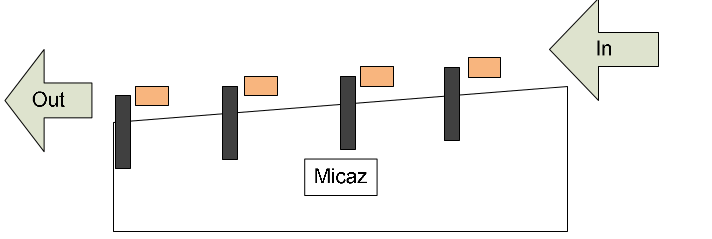
\includegraphics[width=0.9\textwidth]{SkizzeRampe.png}
	\caption{Beispiel einer eingesetzten Rampe}
	\label{fig:skiram}
\end{figure}

\subsubsection{Mikrocontroller}
Ein Mikrocontroller ist ein vollständiger Kleinstrechner auf einem einzigen Chip, dessen Zentraleinheit aus einem oder mehreren Mikroprozessen besteht. Zusätzlich enthält ein Mikrocontroller Speicher und Ein- bzw. Ausgabeschnittstellen zur Außenwelt. Dazu können neben einfach Ausgangspins auch komplexere Busprotokolle wie etwa USART, SPI oder CAN gehören.

Mikrocontroller werden eingesetzt, wenn eine Kommunikations- oder Steuerungsaufgabe mit möglichst geringen Ressourcen (Baugröße, Energie, Kosten) gelöst werden müssen. Die in einem Mikrocontroller verbauten Prozessorkern, Speicher und die Aus- und Eingabeschnittstellen, sind auf die Lösung derartiger Aufgaben zugeschnitten. Die große Anzahl an potenziellen Aufgabenstellungen hat zur Folge, dass es eine Vielfalt von Mikrocontrollern gibt. Meist sind die Mikrocontroller deshalb in Mikrocontrollerfamilien aufgeteilt. Innerhalb einer Familie unterscheiden sich die Controller nicht im Prozessorkern, sondern im verfügbaren Speicher und in den Ein- und Ausgabeschnittstellen \cite{ECHT2005}. In \autoref{fig:aufbmc} ist der schematische Aufbau eines MCs dargestellt.
\begin{figure}[th]
	\centering
		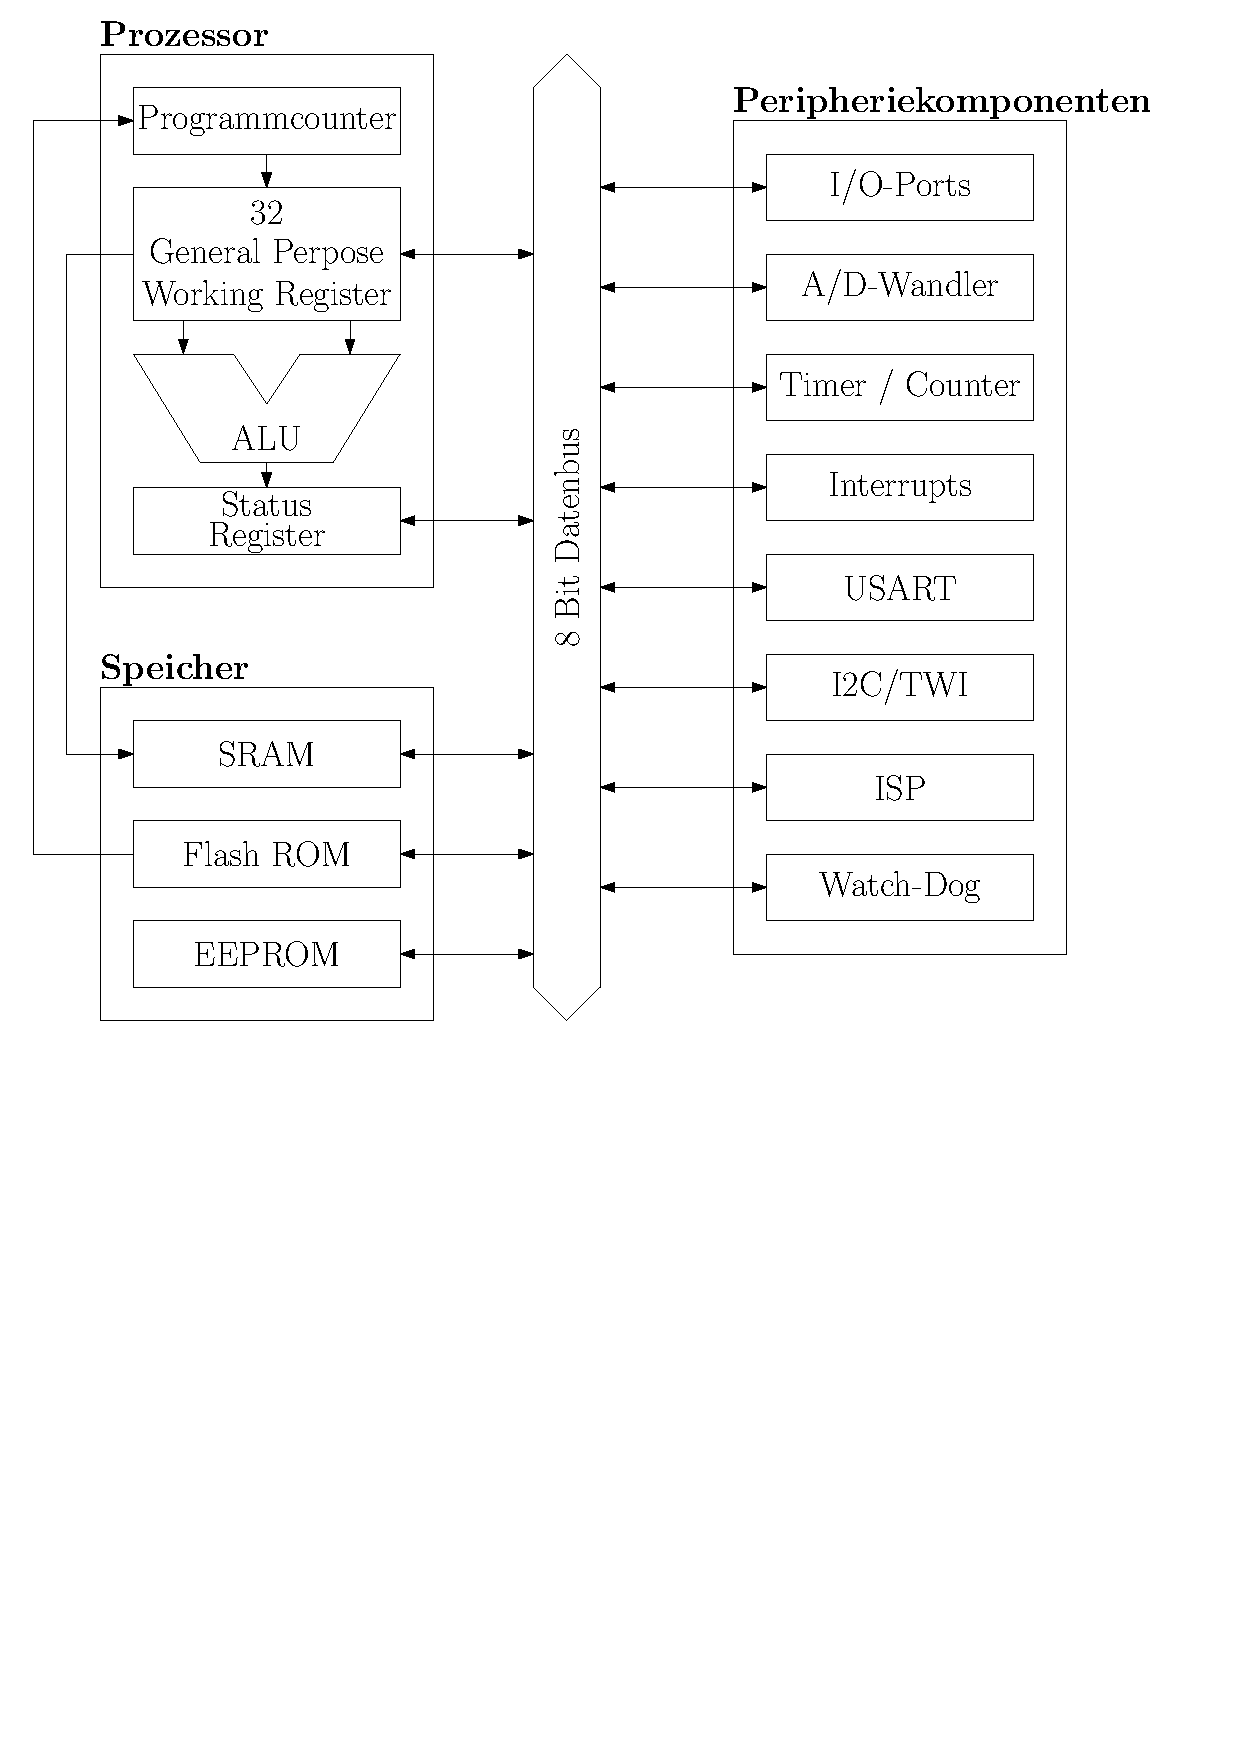
\includegraphics[width=0.8\textwidth]{flow/schemamc.pdf}
	\caption{Schematischer Aufbau eines Mikrocontrollers vgl. \cite{Brinkschulte:2002:Mikrocontroller}}
	\label{fig:aufbmc}
\end{figure}

Die zentrale Steuereinheit eines MCs ist der \textbf{Prozessor} (engl.: Central Processing Unit (CPU)). Sie ist die wichtigste Funktionseinheit und für die Verarbeitung von Befehlen und arithmetischen Berechnungen verantwortlich. Über den internen Bus kann die CPU mit weiteren Grundbausteien kommunizieren und beispielsweise auf Daten innerhalb des Speichers zugreifen.

Der \textbf{Speicher} besteht in der Regel aus dem Arbeitsspeicher (RAM, kurz für: Random Access Memory) und dem Programmspeicher bzw. Flash-Speicher. Normalerweise werden diese zwei Speichertypen logisch voneinander getrennt. Programme werden im nichtflüchtigen Flash-Speicher gesichert. Dieser kann mehrere Kilobyte (KB) bis Megabyte (MB) umfassen. Bei speziellen Systemen ist es möglich den Programmspeicher durch externe Flash-Komponenten zu erweitern um zusätzlichen Speicherplatz zu gewinnen.

Zwischenergebnisse, Messwerte von Sensoren, Steuergrößen usw. werden auf dem RAM abgelegt. Dieser ist deutlich schneller als der Flash-Speicher, verfügt aber in der Regel über deutlich weniger Speicherplatz. Alle Werte, welche zur Laufzeit im RAM abgelegt werden, sind im Gegensatz zum Flash-Speicher flüchtig. Das bedeutet, dass Daten bei einem Neustart des Mikrocontrollers nicht erhalten bleiben.

Durch die \textbf{Peripheriekomponenten} wird die Verbindung und Kommunikation zwischen Controller und Außenwelt ermöglicht. Über die digitalen Ein- und Ausgänge (GPIO, kurz für: General Purpose Input/Output) können Sensoren, Aktoren oder andere Systeme mit dem Mikrocontroller verbunden werden. Die meisten Mikrocontroller bieten eine Vielzahl von Ein- und Ausgängen \cite[S. 13-16]{SOM2012}.

Bei der Umsetzung des Projekts wurden \textsc{Mica}z-Module eingesetzt. Im Folgenden werden kurz die Eigenheiten dieser Module erläutert.

\paragraph{\textsc{Mica}z-Modul}
Ein \textsc{Mica}z-Modul ist drahtloser Sensornetzwerkknoten von der Firma Memsic. Mehrere dieser Module übernehmen in der physischen Zelle die Berechnung Geschäftslogik und die Steuerung der Rampen. \autoref{fig:micaz} zeigt ein solches Modul, während \autoref{fig:blockmicaz}  ein Blockdiagramm von dessen Struktur darstellt. Herzstück der Module ist ein ATMega128L-Mikrocontroller. Bei diesem handelt es sich um einen Low-Power-Mikrocontroller von der Firma Atmel. Darüber hinaus verfügt ein \textsc{Mica}z-Module über einen CC2420-Funkchip der Firma Texas Instruments. Dieser ermöglicht die drahtlose Kommunikation mit anderen Modulen auf einer Frequenz von 2.4 GHz ermöglicht. Es wird dabei der IEEE 802.15.4 Standard verwendet. Eine Antenne kann über eine MMCX-Schnittstelle mit dem Modul verbunden werden, um Signalstärke und -reichweite zu erhöhen. Weiter verfügen die Module über einen 128 KB großen Flash-Speicher.
Zugang zu einee Vielzahl der Leitungen des Moduls gewährt ein 51-poliger Steckverbinder. Über eine Erweiterungsplatine werden so etwa die Lichtschranken und Magnetbolzen der Rampe angeschlossen. Denkbar wäre auch ein größerer Arbeitsspeicher, alle nötigen Pins des Mikrocontrollers sind über den Steckverbinder erreichbar.
Im Projekt wurde die Steckverbindung weiterhin dafür genutzt, die \textsc{Mica}z-Module über ein \textsc{Mib}520 an einen PC anzuschließen, um sie über eine UART-Schnittstelle auszulesen und per JTAG (siehe \autoref{sec:JTAGICE3}) zu programmieren \cite{MICSHEET,C2420SHEET}.

\begin{figure}[th]
  \centering
    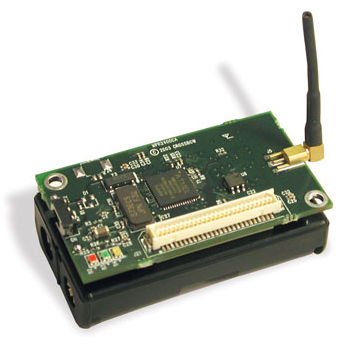
\includegraphics[width = 0.4\textwidth]{flow/micaz.png}
    \caption{\textsc{Mica}z-Modul \cite{Memsic:2014:Online}}
    \label{fig:micaz}
\end{figure}

\begin{figure}[th]
  \centering
    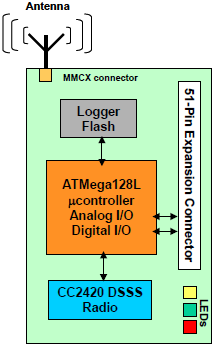
\includegraphics[width = 0.4\textwidth]{flow/blockmicaz.PNG}
    \caption{Blockdiagramm der \textsc{Mica}z-Module  \cite{Memsic:2014:Online}}
    \label{fig:blockmicaz}
\end{figure}

\paragraph{\textsc{Mib}520}
Ein \textsc{Mib}520 stellt eine Schnittstelle für \textsc{Mica}z-Module dar. Es erlaubt die Verbindung eines \textsc{Mica}z-Moduls mit einem Computer per USB-Schnittstelle. So kann über die USART-Schnittstelle des Moduls mit dem PC kommuniziert werden. Über diese Verbindung wurde die Schnittstelle zu den Volksbots realisiert. Weiterhin verfügt ein \textsc{Mib}520-Gateway über eine \textbf{JTAG}-Schnittstelle.


\subsection{Werkzeuge}

\subsubsection{Robot Operating System (ROS)}

Es gibt viele Robotik-Frameworks, die spezifisch für präzise Anwendungen, für Prototypen,
erstellt wurden. ROS strebt da eher das Allgemeine an. Das »Robot Operating System«
(ROS) ist ein Open-Source Framework für individuelle Roboter, das sich in der
Robotikforschung in den letzten Jahren etabliert hat und ein großes Repertoire an Software-Komponenten und -Werkzeugen für Robotikapplikationen bietet.\\
Die Entwicklung begann 2007 am Stanford Artificial Intelligence Laboratory im Rahmen des
Stanford-AI-Robot-Projektes (STAIR). Heute wird es hauptsächlich am Robotik Institut Willow
Garage weiterentwickelt. Seit April 2012 wird ROS von der neu gegründeten,
gemeinnützigen Organisation Open Source Robotics Foundation (OSRF) unterstützt. Die
Bibliotheken von ROS setzen auf Betriebssysteme wie Linux, Mac OS X oder Windows auf.
ROS ist nicht von einer spezifischen Sprache abhängig. Heutzutage gibt es 3 Grundlibraries
für ROS, die jeweils auf Python, Lisp und C++ ausgerichtet sind. Zwei Exmperimentier-
Librairies sind für Java und Lua erhältlich.
\subsubsection*{Was will ROS?}
\begin{itemize}
 \item ROS will unterstützen, Code für Forschung und Entwicklung wiederzuverwenden
 \item loser Verbund von individuellen Programmteilen (Nodes)
 \item einzelne Programmteile können einfach geteilt und verbreitet werden (Packages und Stacks)
 \item ROS stellt Repositories zu Verfügung, um dort Code zu teilen \cite{ROS:2014:Online}
(http://www.ros.org/browse)
\end{itemize}
\subsubsection*{Was kann ROS?}
Die Hauptbestandteile und Hauptaufgaben von ROS sind Hardwareabstraktion; Gerätetreiber; Implementierung 
von viel genutzten Funktionalitäten; Inter-Prozess-Kommunikation; Paket-Management
\subsubsection*{Aufgaben des ROS}
\begin{itemize}
 \item Interprozesskommunikation (IPC)
 \begin{itemize}
\item Problematik der Kommunikation zwischen verschiedenen Systemen des Roboters
\item Sicherheitseinstellung bei der Übertragung
\item Anforderung an die Geschwindigkeit / Schnelligkeit der Kommunikation
\item Koordination von Nachrichten durch zentralen Master
\end{itemize}
\item Paketverwaltung – Packages
\begin{itemize}
 \item ROS ist durch Softwarepakete (sogn. Packages) aufgebaut
 \item Ein Package beinhaltet Laufzeitprozesse (Nodes); ROS abhängige Bibliotheken;
Datensätze; Konfigurationsdateien;3rd Party Software
 \item Packages sind dazu, da um Code wiederverwendbar zu machen
\end{itemize}
\item Paketverwaltung – Stacks
\begin{itemize}
\item Sammlung von Paketen (Packages)
\item Der Sinn ist, dass Stacks die Verteilung und Verwendbarkeit von Code
vereinfachen
\item Meist viele Packages ähnlicher Aufgaben in einem Stack verpackt
\end{itemize}
\item Message (msg)
\begin{itemize}
 \item  Messages werden verwendet um unter ROS Nachrichten zwischen Knoten und
Topics auszutuaschen
\item Dafür verwendet ROS eine einfache Beschreibung der Datentypen in Textdateien
\item Durch diese Beschreibung kann für unterschiedliche Sprachen Code autogeneriert
werden
\item Diese sind in .msg-Dateien im msg- Unterverzeichnis eines ROS-Pakets abgelegt
\item Eigene Message-Typen sind mit Paket Ressource-Namen bezeichnet
\item Standard Messages sind mit std\_msg/msg/String.msg bezeichnet
\end{itemize}
\item Service
\begin{itemize}
 \item ROS verwendet eine eigene vereinfachte Service Description Language ("srv") für die
Beschreibung von ROS Service-Typen
\item Setzt direkt auf die ROS msg-Format auf
\item Ermöglicht die Anfrage / Antwort-Kommunikation zwischen den Knoten
\item Service-Beschreibungen sind in .srv-Dateien im srv- Unterverzeichnis eines Pakets
gespeichert
\item Service-Beschreibungen werden für die Verwendung mit dem Paket Ressource-
Namen bezeichnet
\item Z. B.: wird die Datei robot\_srvs/srv/SetJointCmd.srv als Service
robot\_srvs/SetJointCmd bezeichnet
\end{itemize}
\item Notes
\begin{itemize}
 \item Der Nachrichtenaustausch findet bei Nodes durch 3 Möglichkeiten statt: Parameter
Server;Topics; Services
\item Nodes werden wie in einem Graph angeordnet
\item In einem System laufen viele Nodes Parallel
\item Diese werden zu Beginn gestartet
\item Beispiele sind Nodes für: Laserscanner; Kinect; Pfadplanung
\end{itemize}
\item Topica
\begin{itemize}
 \item Topics verhalten sich wie ein virtuelles BUS-System Nodes können von Topics lesen
(subscribe)
\item Nodes können an Topics senden (publish)
\item Es gibt keine Begrenzung wie viele Nodes publsih oder subscribe auf ein Topic
machen
\end{itemize}
\end{itemize}
\subsubsection*{ROS-Datensystem}
ROS-Ressourcen sind in rangmäßiger Gliederung eingeordnet. Zwei Konzepte sind zu
verstehen:
\begin{itemize}
\item \textbf{Le package}: Es handelt sich hier um die Zentraleinheit der Softwareorganisation von
ROS. Ein Package ist ein Verzeichnis der die Knoten beinhaltet (wir werden hier
unten erklären, was ein Knoten ist) sowie die externen Librairies, Daten und XML
Konfigurationsdateien die manifest.xml genannt wird.
\item \textbf{Stack}: Stack bezeichnet eine Sammlung von Packagen. Sie ermöglicht mehrere
Funktionen wie Navigation, Lokalisierung und viele mehr. Ein Stack beinhaltet
mehrere Verzeichnisse sowie eine Konfigurationsdatei die stack.xml genannt wird.
\begin{itemize}
\item Vorhandene wichtige Stacks
\begin{itemize}
\item TF – Koordinatentransformation
\item Navigationstack
\item URDF - Modelle
\end{itemize}
\begin{itemize}
\item Beispiel Navigationstack
\begin{itemize}
\item Wertet Sensordaten aus z.B.: Laserdaten
\item Baut daraus mit gmapping (ebenfalls ein ROS-Stack) eine Begehbarkeitskarte
\item Warum? Zur Kollisionsvermeidung
\item Bei erfolgreicher Erstellung einer Map kann dann ein Ziel übergeben werde (Pfadplanung durch Navigationstack,
Kollisionsvermeidung, Reaktion auf sich ändernde Umgebung, Aufbau einer globalen Karte)
\end{itemize}
\end{itemize}
\end{itemize}
\end{itemize}
\subsubsection*{Vorteile und Nachteile des ROS}
\paragraph*{Vorteile}
\begin{itemize}
 \item Nachrichten-basierte Software Architektur
\begin{itemize}
\item Verschiedene Komponenten sind unabhängig voneinander mit dem System verbunden
\item Unterschiedliche Komponenten können miteinander verbunden werden, ohne jedes Mal das Programm neu zu Kompilieren
\item Netzwerkfähigkeit
\item Einfaches Debugging und Simulieren
\end{itemize}
\item Absturz eines Nodes führt nicht zum Absturz des ganzen
Systems
\item Für ROS lässt sich in mehreren Sprachen programmieren
\item ROS hat eine große Community, die viele Daten und Programme zu Verfügung
stellen
\end{itemize}
\paragraph*{Nachteile}
\begin{itemize}
 \item Durch Nachrichten-basierte Systemarchitektur Bottleneck bei großer Datenmenge
\item Steuerung des Systems über Kommandozeile
\end{itemize}

\subsubsection{Epos Control}

\subsubsection{SOPAS Engineeringtool}

Bei SOPAS ET handelt es sich um ein Entwicklungsprogramm von Sick. Dieses wird zur Ansteuerung und Konfiguration der Laserscanner und Hallsensosren verwendet.

\begin{itemize}
\item \textbf{ Erster Start }

Beim ausführen von SOPAS wird ein neues Projekt erstellt, in dem man die gewünschte Hardware selektiert und einbindet. Die Wahl der Hardware erfolgt hierbei über den Netzwerkscanassistenten oder manuell über den Gerätekatalog. Sobald die Kommunikation mit der Hardware aktiv ist, kann diese angesteuert werden. Änderungen der Konfiguration der Hardware sind im Projektbaum möglich oder sogar notwendig ( siehe Kapitel 7.7 Herausforderungen).
\end{itemize}


\subsection{Systemarchitektur}

\subsubsection{Contiki}
Contiki ist ein Open Source Echtzeitbetriebssystem, das bei uns in der PG auf den MICAz-Modulen eingesetzt wird.
Contiki bietet einen einfachen ereignisgesteuerten Betriebssystemkern mit sogenannten Protothreads, optionalem 
pr\"aemptiven Multiprogramming, Interprozesskommunikation via Messagepassing durch Events, eine dynamische Prozessstruktur
mit Unterst\"utzung f\"ur das Laden und Entladen von Programmen, nativen TCP/IP-Support über den uIP TCP/IP-Stack und eine 
grafische Benutzerschnittstelle, welche direkt auf einem Bildschirm oder als virtuelle Anzeige \"uber Telnet oder VNC genutzt werden kann \cite{Wikipedia:2013:Online}.
 
\paragraph{Systemarchitektur}
Ein laufendes Contiki System besteht aus dem Kernel, Bibliotheken, Prozessen und dem Programm-Lader, mit dem Anwendungen zur Laufzeit aus dem Speicher oder \"uber ein Funkmodul geladen werden k\"onnen.
Die unten stehende Abbildung zeigt die Aufteilung des Betriebssystems in zwei Teile. 
\begin{figure}[h!]
	\centering
		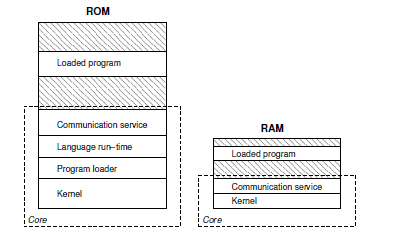
\includegraphics[width=0.9\textwidth]{Systemarchitektur_Contiki.png}
	\caption{Komponenten von Contiki \cite{Dunkels:Groenvall:Voigt:2014:Online}}
	\label{Systemarchitektur von Contiki}
\end{figure}
Der Core ist ein Basissystem und besteht aus dem Kernel, Bibliotheken, Ger\"{a}tetreibern und dem Programm-Lader. 
Im allgemeinen sind \"Anderungen am Core nicht vorgesehen und nur unter Verwendung eines speziellen Bootloaders m\"oglich. 
Die konkrete Aufteilung des Systems in Core und ladbare Programme wird beim Kompilieren des Systems entschieden und h\"angt 
von der Hardware-Plattform ab \cite[vgl.][S. 7]{Walter:2010}. Ger\"atetreiber werden als Bibliotheken implementiert. 

\paragraph{Events}
In Contiki kommunizieren Prozesse \"uber Events. Auch der Kernel versendet Events, um Prozesse \"uber ihren Status 
(Init, Continue, Exit) oder \"uber abgelaufene Timer zu Informieren. Zur Identifikation stehen dabei Event IDs zur 
Verf\"ugung. Die Event IDs 0-127 k\"onnen vom Benutzer frei vergeben werden, w\"ahrend die Prozess IDs ab 128 vom 
System genutzt werden. Grunds\"atzlich unterscheidet Contiki zwischen synchronen und asynchronen Events. 
\begin{itemize}
\item \textbf{Asynchrone Events} sind eine Form der Deferred Procedure Call: asynchrone Events werden vom Kernel in einer 
Warteschlange gespeichert. Die Scheduling-Funktion des Kernels l\"auft nach Systemstart in einer Endlosschleife. 
In jedem Durchlauf wird ein Event aus der Schlange entnommen und wird einige Zeit sp\"ater an den Zielprozess weitergeleitet.
\item \textbf{Synchrone Events} gleichen einem Funktionsaufruf.
Sie werden ohne Umweg \"uber die Warteschlange direkt an den Empf\"anger-Prozess
zugestellt \cite[vgl.][S. 7]{Walter:2010}.  Mit der Funktion process\_post\_synch(\&example\_process, EVENT\_ID, msg) wird gezielt ein 
Prozess aufgerufen (ein Broadcast ist nicht m\"oglich). W\"ahrend der aufgerufene Prozess aktiv ist, blockiert der Aufrufer und 
setzt seine Ausführung erst fort, wenn der aufgerufene Prozess die Kontrolle wieder abgibt.
\end{itemize}

\paragraph{Prozesse}
Prozesse in Contiki implementieren ein Konzept namens Protothreads. Dies erlaubt es Prozessen, ohne den Overhead und die langen 
Prozesswechselzeiten von normalen Threads auszukommen. Gleichzeitig k\"onnen trotzdem andere Prozesse ausgef\"uhrt werden, falls ein Prozess auf ein Event (Timer, Nachricht von anderem Prozess...) warten muss.
F\"ur die Entwicklung mit Prozessen ist wichtig, dass nicht-statische Variablen nicht zwischen zwei Aufrufen erhalten bleiben.
Der relevante Status eines Prozesses sollte daher mithilfe von statischen Variablen abgelegt werden (siehe Variable i im folgenden Beispiel)

\begin{figure}[h!]
	\centering
		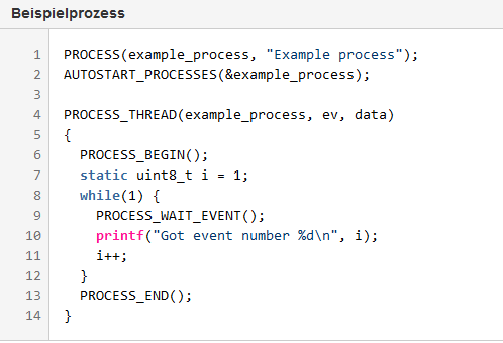
\includegraphics[width=0.9\textwidth]{Beispielprozess.png}
	\label{Beispielprozess}
\end{figure}
In Zeile 1 wird der Prozess initialisiert und in Zeile 2 automatisch beim Boot von Contiki gestartet. Zeile 4 beinhaltet die
Deklaration. So k\"onnen andere Prozesse diesem Prozess Events (mit oder ohne Daten) schicken, auf die unser Beispielprozess 
mit ev und data zugreifen kann. Zeile 6 kennzeichnet den Beginn der tats\"achlichen Ablauflogik. Code \"uber dieser Zeile wird 
bei jedem Prozessaufruf ausgef\"uhrt, dies wird jedoch in den meisten F\"allen nicht ben\"otigt. Zeile 13 schlie{\ss}lich beendet
den Prozess und entfernt ihn aus der Prozess-Liste des Kernels. In diesem Beispiel wird die Zeile jedoch nie erreicht, sodass der Prozess immer wieder aufgerufen wird, bis er von einem anderen Prozess beendet wird.
Wichtige Funktionen in Prozessen:
\begin{itemize}
\item PROCESS\_WAIT\_EVENT() - Wartet auf ein beliebiges Event, bevor die Ausf\"{u}hrung fortgesetzt wird.
\item PROCESS\_WAIT\_EVENT\_UNTIL(condition) - Wartet auf ein beliebiges Event, setzt die Ausf\"{u}hrung aber nur fort, wenn die Bedingung erf\"{u}llt ist.
\item PROCESS\_WAIT\_UNTIL() - Wartet, bis die Bedingung erf\"ullt ist. Muss den Prozess nicht zwangsl\"{a}ufig anhalten.
\end{itemize}
Prozesse k\"onnen \"uber Events (siehe Events) oder Polling-Anfragen kommunizieren.  Polls sind Events mit hoher Priorit\"at und 
k\"onnen genutzt werden, um den angerufenen Prozess so schnell wie m\"oglich auszuf\"uhren. Sie
sind besonders bei der Abarbeitung von Hardware-Interrupts wichtig, da Interrupts-Handler keine Events, sondern nur
Polling-Anfragen absetzten d\"urfen \cite[vgl.][S. 7]{Walter:2010}.

\subsubsection{Background Level: Treiber, Services und Interfaces}
Im Background Level werden Teiber, die sich um die Schnittstellen/Pins des Controllers wie z.~B. Protokolle angeschlossener Devices\cite[S. 26]{Stasch:Hahn} kümmern, Services, deren Aufgabe es ist, die Funktionen der Treiber zu sinnvollen Einheiten zusammenzufassen, und schließlich Interfaces, die genutzt werden, um die Funktionen der Services dem AgentenRTE zur Verfügung zu stellen und gleichzeitig plattformabhängige Implementierungsdetails zu maskieren, implementiert \cite[S. 26]{Stasch:Hahn}. Im Laufe der Projektarbeit wurden unterschiedliche Treiber, Services und Interfaces entwickelt. Der folgende Abschnitt soll diese einzeln näher beleuchten.

\paragraph{Treiber Bolzen}
Folgende Funktionen werden im Treiber für die Bolzen bereitgestellt:
\begin{itemize}
  \item void BoltDriver\_init(void)
  \item void BoltDriver\_up(unsigned char boltv)
  \item void BoltDriver\_down(unsigned char boltv)
  \item uint8\_t BoltDriver\_get(void)
\end{itemize} 
Die Funktion \textit{void BoltDriver\_init(void)} dient zur Initialisierung. Dabei werden die Ports der \textsc{Mica}z-Module, die für die Bolzensteuerung nötig sind, als Ausgänge festgelegt und gleichzeitig auf HIGH-Aktiv gesetzt.

Zum Öffnen der Bolzen wird die Funktion \textit{void BoltDriver\_down(unsigned char boltv)} genutzt. Ihr wird ein Vektor übergeben, der die Pinbelegung von den zu öffnenden Bolzen enthält. Da die Bolzen beim öffnen jeweils eine Anfansspannung von 24 Volt benötigen, muss darauf geachtet werden, dass die Bolzen nacheinander geöffnet werden. Im ersten Schritt fragt die Funktion ab, ob Bolzen 1 geöffnet werden soll. Bei erfolgreicher Prüfung, werden Pin 1 und 2 der ersten Bolzen angeschaltet, wodurch eine Anfangsspannung von 24 Volt anliegt und der Bolzen sich öffnen kann. Damit das Öffnen erfolgreich sichergestellt werden kann, wird dieser Zustand über 60 Taktzyklen gehalten, dann wird der zweite Pin wieder ausgeschaltet. Jetzt liegen über den angeschlossenen Verstärker noch 12 Volt Spannung an, was ausreicht um den Bolzen offen zu halten, ohne die Schaltung zu überhitzen. Im nächsten Schritt wird überprüft ob beide Bolzen gleichzeitig geöffnet werden sollen. Ist dies der Fall, dann wird wieder für 60 Taktzyklen im System gewartet. Im Anschluss daran wird kontrolliert, ob Bolzen 2 geöffnet werden soll. Liegt hier eine positive Bewertung vor, wird mit den Pins von Bolzen 2 analog zu Bolzen 1 vorgegangen.

Die Funktion \textit{void BoltDriver\_up(unsigned char boltv)} schließt die Bolzen. Dieser Funktion wird ebenfalls ein Vektor übergeben, der die Belegung der Bolzen enthält, die geschlossen werden sollen. Dabei wird geprüft, welche Bolzen geschlossen werden sollen. Anschließend werden dann jeweils beide Pins der Bolzen auf LOW gezogen, ein sukzessives \textit{Herunterfahren} der Spannung wie beim Öffnen ist nicht nötig.

Mit der Funkion \textit{uint8\_t BoltDriver\_get(void)} kann die Bolzenstellung abgefragt werden. Dabei wird einfach überprüft, ob die Ausgänge des \textsc{Mica}z-Modul an denen die Bolzen angeschlossen sind HIGH sind. Beim Rückgabevektor steht eine Eins im Vektor für einen offenen und eine Null für einen geschlossenen Bolzen.

\paragraph{Interface Bolzen}
Das Bolzen-Interface greift direkt auf die Treiber der Bolzen zu und stellt mehrere Funktionen zur Verfügung, durch die Prozesse gestartet werden. Die unterschiedlich bereitgestellten Funkionen im Bolzen-Interface sind:
\begin{itemize}
  \item void BoltInterface\_init(void);
  \item void BoltInterface\_release(void);
  \item void BoltInterface\_release\_and\_separate(void);
  \item void BoltInterface\_separate(void);
\end{itemize}

Durch die unteren drei Funktionen werden folgende Prozesse gestartet:
\begin{itemize}
  \item PROCESS\_NAME(bolt\_int\_release)
  \item PROCESS\_NAME(bolt\_int\_release\_and\_separate)
  \item PROCESS\_NAME(bolt\_int\_separate)
\end{itemize}

Der Prozess \textit{bolt\_int\_release} ist dafür zuständig, die untersten zwei Bolzen für einen bestimmten Zeitraum zu öffnen und dann wieder zu schließen. Dafür existieren zwei Zustände. Im ersten Zustand wird die Funktion \textit{BoltDriver\_up(unsigned char boltv)} aufgerufen. So wird sichergestellt, dass die oberen beiden Bolzen geschlossen sind, um nur exakt ein Paket freizugeben. Nach dem Aufruf der Funktion wird ein Timer gestartet. Zustand zwei ruft, sobald der Timer abläuft, die Funktion \textit{BoltDriver\_down(unsigned char boltv)} aus dem Treiber mit einem Vektor für die unteren beiden Bolzen auf und das Paket wird freigegeben. Im Anschluss daran, wird wieder ein Timeout gesetzt und gewartet. Nach dem Durchlauf der zwei Zustände wird vorm Prozessende die Funktion \textit{BoltDriver\_up(unsigned char boltv)} aus den Treibern aufgerufen, um die unteren Bolzen wieder zu schließen.

Um Pakete nicht nur von der Rampe auszugeben, sondern auch gleich das nächste Paket zu separieren, ist der Prozess \textit{bolt\_int\_release\_and\_separate} zuständig. Dabei werden zu Anfang des Prozesses vier unterschiedliche Zustände durchlaufen. Die ersten drei Zustände sind dafür da, das Paket von der Rampe zu entfernen. Hierbei wird genau wie oben beim der Funktion \textit{bolt\_int\_release} vorgegangen. Zustand vier wird im Anschluss daran dann benutzt, die oberen Bolzen wieder zu öffnen, damit das nächste Paket nachrutschen kann. Vorm Abschluss des Prozesses werden diese dannn wieder durch die Treiberfunktion \textit{BoltDriver\_up(unsigned char boltv)} geschlossen.

Mit dem dritten Prozess wird es ermöglicht, die oberen zwei Bolzen zu öffnen. Beim Prozessdurchlauf wird im Zustand eins sichergestellt, dass die unteren beiden Bolzen geschlossen sind. Im zweiten Zustand werden dann die oberen zwei Bolzen geöffnet, was ein Nachrutschen von Paketen ermöglicht. Bevor der Prozess dann beendet wird, werden die beiden Bolzen wieder geschlossen. Der Prozess ermöglicht es somit, ein Paket zu separieren.

\paragraph{Treiber Externer Speicher}
\label{sec:externalMemory}
Der Treiber für den externen Speicher setzt den SPI-Bus zum AT45DB041-Chip um. Dafür nutzt er die Pins D2 (RXD oder SO), D3 (TXD oder SI), D5 (SCK) und A3 (CS). Ein Befehl an den Speicher ist dabei stets gleich aufgebaut:
\begin{itemize}
\item 1 Byte Opcode
\item 4 Don't-Care-Bits und 11 Bit Seiten-Adresse
\item 9 Bit Buffer-Adresse
\item Read Trigger (nur für Lese-Befehle, Senden von ebenso vielen leeren Bytes wie empfangen werden sollen)
\end{itemize}

Der Treiber stellt folgende Funktionen zur Verfügung:

\begin{itemize}
  \item void ExtflashDriver\_init()
  \item uint8\_t ExtflashDriver\_tr\_byte(uint8\_t spiOut)
  \item void ExtflashDriver\_enable()
  \item void ExtflashDriver\_disable()
  \item void ExtflashDriver\_wait\_idle()
  \item uint8\_t ExtflashDriver\_read\_status\_register(void)
  \item uint8\_t ExtflashDriver\_get\_last\_compare(void)
\end{itemize}

Bemerkenswert ist hier insbesondere die Funktion \textit{ExtflashDriver\_tr\_byte}. Entsprechend des SPI-Busses sendet und empfängt sie gleichzeitig ein Byte vom Speicher.  \textit{ExtflashDriver\_wait\_idle} empfängt das erste Byte des Statusregisters. So kann geprüft werden, ob der Speicherchip gerade eine Seite in den Buffer lädt oder den Buffer zurückschreibt und deshalb mit dem nächsten Befehl gewartet werden muss \cite{AT45DB041A:2014:Online}.
\paragraph{Interface Externer Speicher}
Das Interface stellt für das Speicherinterface folgende Funktionen zur Verfügung:
\begin{itemize}
  \item void ExtflashInterface\_init()
  \item void ExtflashInterface\_restore(uint16\_t cell)
  \item void ExtflashInterface\_flush(uint16\_t cell)
  \item void ExtflashInterface\_agent\_restore(uint8\_t localAgentId)
  \item void ExtflashInterface\_agent\_flush(uint8\_t localAgentId)
  \item uint8\_t ExtflashInterface\_write(uint16\_t address, uint8\_t* data, uint8\_t len)
  \item uint8\_t ExtflashInterface\_read(uint16\_t address, uint8\_t* data, uint8\_t len)
\end{itemize}
\textit{ExtflashInterface\_restore} holt zwei aufeinanderfolgende Seiten (eine Zelle) aus dem Speicher und schreibt sie in den Buffer. \textit{ExtflashInterface\_flush(uint16\_t cell)} schreibt die beiden Seiten im Buffer an die angegebene Stelle im Speicher. \textit{ExtflashInterface\_agent\_restore} und \textit{ExtflashInterface\_agent\_flush} holen die Zelle eines bestimmten Agenten in den Speicher und schließlich sind \textit{ExtflashInterface\_write} und \textit{ExtflashInterface\_read} für Datenzugriffe im Buffer zuständig und können Daten lesen beziehungsweise schreiben.
\paragraph{Speicherinterface}
Das Speicherinterface stellt den Agenten den externen Flashspeicher zur Verfügung. Jedem Agenten werden dafür zwei Seiten zugeordnet. Ruft er nun die Funktionen \textit{MemoryInterface\_readComponentCell(uint8\_t componentCount, uint8\_t cell, uint8\_t* result, uint8\_t length)} oder \textit{MemoryInterface\_writeComponentCell(uint8\_t componentCount,uint16\_t cell, uint8\_t* data, uint8\_t length)} auf, wird geprüft, ob die Zelle des aktuellen Agenten bereits im Buffer ist. Falls nicht, werden die aktuellen Bufferdaten gesichert und es werden die Daten des aktiven Agenten geladen.
\paragraph{Treiber Lichtschranken}
Durch den Lichtschrankentreiber werden zwei Funktionen zur Verfügung gestellt. Zum einen ist es die Funktion \textit{void photosensor\_drv\_init(void)}. In dieser werden alle nötigen Eingänge der \textsc{Mica}z-Module initialisiert. Zum anderen wird durch den Treiber die Funktion \textit{uint8\_t get\_photosensors()} implementiert. Durch die Funktion kann der Zustand der Lichtschranken abgefragt werden. Dabei steht eine 1 für eine unterbrochene und eine 0 für eine offene Lichtschranke.

\paragraph{Interface Lichtschranken}
Über das Interface zur Lichtschranke werden folgende drei Funktionen bereitgestellt:
\begin{itemize}
  \item void PhotosensorInterface\_init(void)
  \item uint8\_t PhotosensorInterface\_is\_bay\_occupied(uint8\_t i)
  \item uint8\_t PhotosensorInterface\_num\_packages(void)
\end{itemize}
Durch die Funktion \textit{void PhotosensorInterface\_init(void)} werden die Lichtschranken über den Treiber initialisiert. Dafür wird lediglich die Funktion \textit{void photosensor\_drv\_init(void)} aus dem Treiber aufgerufen.

Die zweite oben aufgeführt Funktion wird genutzt, um zu überprüfen, ob eine bestimmte Lichtschranke unterbrochen wurde oder nicht. Dafür wird der Funktion ein Wert übergeben, der die zu überprüfende Lichtschranke enthält. Ist der übergebende Wert größe als vier, mehr Lichtschranken wurden nicht verbaut, oder kleiner als eins wird eine 0 zurückgegeben, was als nicht ausgelöste Lichtschranke zu interpretieren ist.

\paragraph{Treiber Funkmodul}
Der Treiber für das Funkmodul ist zuständig für die korrekte Funktionalität der drahtlosen Kommunikation zuständig und greift dafür auf den Contiki-Kommunikationsstack \textit{RIME} zu. Auf das Coktiki-interne Atomic Broadcast Protokoll wird durch den Treiber ein Networkflooding augesetzt, das eine zuverlässigere Nachrichtenübermittlung ermöglicht. Dabei werden folgende Funktionen zur Verfügung gestellt:\begin{itemize}
  \item void radio\_open(struct radio\_conn *c, uint16\_t channel, const struct radio\_callbacks *u)
  \item void RadioDriver\_sendmessage(uint8\_t* msgtext, uint8\_t length)
  \item void RadioDriver\_receivemessage(struct radio\_conn *c)
  \item void RadioDriver\_init(void)
\end{itemize}


\paragraph{Treiber UART-Schnittstelle}
Der UART-Treiber ermöglicht die Kommunikation der \textit{Mica}z-Module über den USB-Port. Dafür wurden vom Treiber die folgenden Funktionen entwickelt.
\begin{itemize}
  \item void UartDriver\_send(uint8\_t *buf, uint8\_t size)
  \item int UartDriver\_line\_input\_byte(unsigned char c)
  \item void UartDriver\_line\_init(void)
\end{itemize}
und zusätlich der Prozess
\begin{itemize}
  \item UartDriver\_recv\_process
\end{itemize}

Die Initialisierung der UART-Schnittstelle findet in der Methode \textit{void UartDriver\_line\_init(void)} statt. Dabei wird ein Ringbuffer, der für den Empfang der Zeichen zuständig ist, initialisert. Außerdem wird der für die Verarbeitung verantwortliche Prozess gestartet.

Die Funktion \textit{void UartDriver\_send(uint8\_t *buf, uint8\_t size)} wird für das Senden über die UART-Schnittstelle benötigt. Dabei wird ein Zeiger auf die Adresse der zusendende Nachricht und die Länge der Nachricht an die Funktion übergeben. Zu Anfang der Funktion wird geprüft, ob die zu sendende Nachricht kleiner als fünf Byte ist. Wenn die Nachricht kürzer als fünf Byte ist, dann wird die Nachricht mit Bytes mit dem Wert 0x00 aufgefüllt. Die Nachricht wird dann byteweise über die UART-Schnittstelle ausgegeben.

Die Methode \textit{int UartDriver\_line\_input\_byte(unsigned char c)} wird zum einlesen über die UART-Schnittstelle verwendet. Es handelt sich hierbei um einen Callback, der von einem Interrupt immer dann aufgerufen wird, wenn ein Byte empfangen wird. Dafür wird überprüft, ob ein Überlauf vorliegt. Wenn dies der Fall ist, wird das Zeichen komplett bis zum Zeilenende ignoriert und der Parameter für den Überlauf auf 0 gesetzt. Wenn genug Platz im Buffer vorhanden ist, wird das empfangene Zeichen eingelesen und im Buffer gespeichert. Kann das Zeichen nicht mehr gespeichert werden, wird der Parameter für den Überlauf auf 1 gesetzt. Zum Schluss wird der Prozess \textit{UartDriver\_recv\_process} gepollt. Dieser ist für die Verarbeitung der empfangenen Nachricht verantwortlich. Dabei wird das eingehende Byte in einen Buffer geschrieben. Wenn der Buffer eine Länge von fünf Byte hat, wird dieser an das Communication Interface weitergereicht.

\paragraph{Interface UART-Schnittstelle}
Durch das UART-Interfache werden folgende Funktionen zur Verfügung gestellt:
\begin{itemize}
  \item void UARTInterface\_drive\_to\_entry(uint16\_t rampid)
  \begin{itemize}
    \item Gibt den Befehl aus, zum Eingang der Rampe mit der Rampen-ID rampid zu fahren
  \end{itemize}
  \item void UARTInterface\_drive\_to\_exit(uint16\_t rampid)
  \begin{itemize}
    \item Gibt den Befehl aus, zum Ausgang der Rampe mit der Rampen-ID rampid zu fahren
  \end{itemize}
  \item void UARTInterface\_how\_cost\_job(uint16\_t startid, uint16\_t targetid)
  \begin{itemize}
    \item Stellt die Frage, wie hoch die Kosten sind ein Paket von Startrampe (startid) zur Zielrampe (targetid)
  \end{itemize}
  \item void UARTInterface\_give\_package(void)
  \begin{itemize}
    \item Befehl Paket an die Rampe abzugeben
  \end{itemize}
  \item void UARTInterface\_take\_package(void)
  \begin{itemize}
    \item Befehl Paket von Rampe entgegenzunehmen
  \end{itemize}
\end{itemize}
Alle Funktionen sind dazu nötig um Befehle an die Teilgruppe Drive zusenden. Mit diesen können Nachrichten an den Volksbot über die USB-Schnittstelle versandt werden.

\subsubsection{Agenten RTE}
\label{sec:AgentRTE}
Auf der nächsten Hierarchieebene über den Interfaces liegt die Laufzeitumgebung der Agenten (AgentRTE). Es ist die erste plattformunabhängige Ebene über den Interfaces und dem Betriebssystem. Vergleicht man die Implementation für STASH-Controller und \textsc{Mica}z-Module, unterscheidet sich das AgentenRTE lediglich im Prozessmodell der Agenten, das abhängig vom Betriebssystem ist: Während die STASH-Controller mit dem MSP430-Mikrocontroller auf SYS/BIOS mit präemptivem Scheduling stetzen, läuft auf den \textsc{Mica}z-Modulen ein nicht-präemptives Contiki-System. Die Agenten auf den Stash-Controllern werden daher jeweils durch einen eigenen Prozess repräsentiert, während es auf den \textsc{Mica}z-Modulen einen gemeinsamen Prozess gibt, der Agenten über Funktionszeiger aufruft. Wir gehen hier nur auf die Implementierung auf den \textsc{Mica}z-Modulen ein.

Neben dem Aufruf der einzelnen Agenten ist das AgentenRTE auch für das Registrieren und Terminieren der Agenten und den Austausch beziehungsweise die Verteilung von Nachrichten verantwortlich.

\paragraph{Verwaltung der Agenten}\mbox{}\\
Agenten werden mit ID und Typ registriert. Nach Konvention bekommt dabei der Plattform-Agent stets die ID des Moduls, der Order-Agent eine um eins erhöhte ID und der Routing-Agent eine um zwei erhöhte ID. Hat Beispielsweise das Modul die ID \textit{0x0110}, so hat der Plattform-Agent ebenfalls die ID \textit{0x0110}, der Order-Agent die ID \textit{0x0111} und der Routing-Agent schließlich die ID \textit{0x0112}. Die Registrierung dieser Agenten erfolgt in der Main-Methode des Systems. Die Nummerierung der Paket-Agenten ist unabhängig von dieser Konvention, allerdings muss darauf geachtet werden, dass ihre IDs nicht mit den übrigen Agenten übereinstimmen.

Registrierte Agenten werden in ein Array aus Agenten-Strukturen eingetragen und dort verwaltet.
\autoref{lst:agentstruct} zeigt die Agenten- und Agenten-Callback-Strukturen. Außerdem wird einmalig ihre Init-Methode aufgerufen.

Bei der Ausführung wird nun bei jedem Prozessaufruf des Agenten-Prozesses eine Zählervariable erhöht, die jeweils die Main-Methode des nächsten Agenten aufruft. Da  Contiki ein nicht-präemptives Scheduling nutzt, dürfen die Agenten nicht blockieren, sondern müssen die Kontrolle an den Haupt-Prozess zurückgeben, sprich die Main-Methode muss terminieren.

\lstinputlisting[language=C, style=customc, captionpos=b, caption={Agenten Strukturen in C}, label=lst:agentstruct]{src/flow/lst/agent_struct.lst}

\paragraph{Austausch von Nachrichten}\mbox{}\\
Der Austausch von Nachrichten und damit die Kommunikaion zwischen Agenten ist unerlässlich in einem Multiagentensystem. Auch diese Aufgabe kommt dem AgentenRTE zu. Die Laufzeitumgebung prüft den Empfänger einer Nachricht und übergibt sie schließlich an den richtigen Agenten. Der Aufbau einer solchen Agenten-Nachricht wird durch eine Struktur beschrieben, die in \autoref{lst:commsg} abgebildet ist. Der Kopf einer Nachricht ist demnach 15 Byte groß, die Nutzdaten können bis zu 26 Byte betragen.

\lstinputlisting[language=C, style=customc, captionpos=b, caption={Struktur einer Agenten-Nachricht in C}, label=lst:commsg]{src/flow/lst/message_struct.lst}

Sendet ein Agent eine solche Nachricht, übergibt er sie dem AgentRTE. Dieses prüft, ob sich der Empfänger-Agent auf dem eigenen Modul befindet. Ist das der Fall, wird die Nachricht in der Warteschlange für eingehende Nachrichten gespeichert und kann dort vom Empfänger abgerufen werden. Wenn der Agent nicht auf der Plattform registriert ist, wird die Nachricht an das CommunicationInterface weitergeleitet, das sich zum die Verteilung im Netzwerk kümmert. So gelangt die Nachricht auch über die Modulgrenzen hinweg zum richtigen Agenten.

Eingehende Nachrichten werden vom CommunicationInterface an das AgentRTE weitergereicht. Dafür wird zunächst angefragt, ob sich der Ziel-Agent beziehungsweise einer der Ziel-Agenten im Falle von Gruppennachrichten auf der Plattform befindet. Ist dies der Fall wird die Nachricht in der Warteschlange für eingehende Nachrichten gespeichert.

Ein großes Problem bei Nachrichtenaustausch stellt der mit 4 KB sehr begrenzte Arbeitsspeicher der \textsc{Mica}z-Module dar. Entsprechend ist der Platz in der Warteschlange für eingehende Nachrichten begrenzt, pro Agent können nur drei Nachrichten gespeichert werden. Um den Speicher nicht überlaufen zu lassen und dadurch Nachrichten zu verlieren, wird daher das Senden von Nachrichten durch ein Token-System begrenzt. Pro Agent kann so in jedem Durchlauf nur eine Nachricht versendet werden. Nutzt ein Agent dies nicht aus, kann sein Token auf einen anderen Agenten übertragen werden. In der Praxis schränkt diese Restriktion die Agenten in ihrer Funktionalität jedoch nicht ein. Meist erfordert eine eingehende Nachricht nur eine direkt Antwort oder die Benachrichtigung eines anderen Agenten. Müssen einmal doch zwei oder mehr Nachrichten als Reaktion versendet werden, geschieht dies mithilfe von Zwischenzuständen und Flags, die beim nächsten Durchlauf aktiv werden.
%\begin{figure}[h!]
%	\centering
%		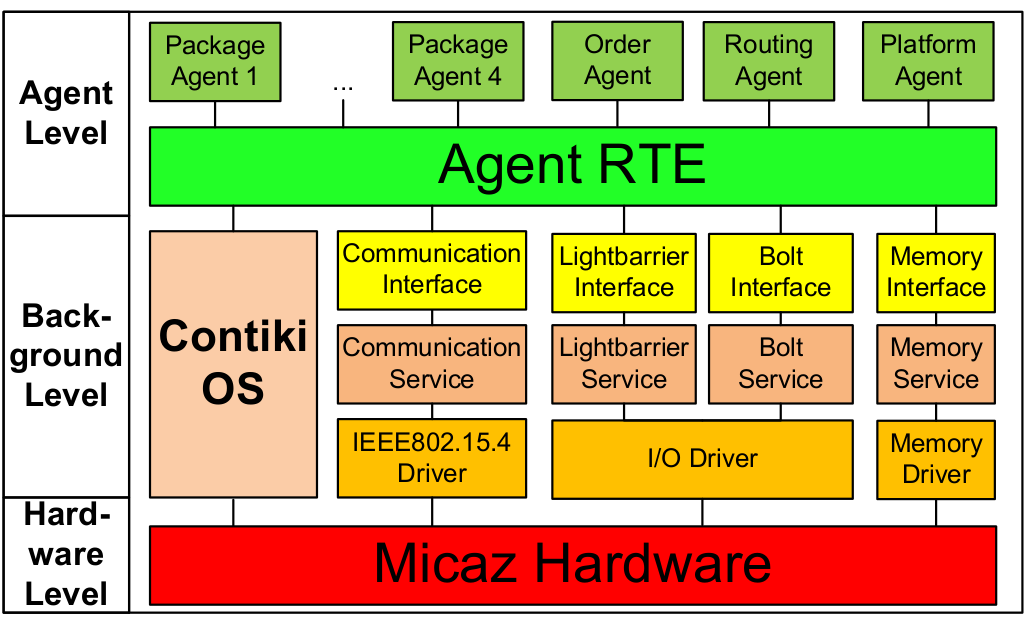
\includegraphics[width=0.9\textwidth]{ArchitekturMicazRampe.png}
%	\caption{Architektur Micaz Rampe\cite{Stasch:Hahn}}
%	\label{ArchitekturMicazRampe}
%\end{figure}

\subsection{Agenten}
Oberhalb des AgentRTE sind die Agenten implementiert. Sie bilden die oberste Ebene des Systems und implementieren die eigentliche Funktionalität. Dabei greifen sie auf das AgentenRTE und die verschiedenen Interfaces zu und kommunizieren untereinander über Agenten-Nachrichten. Auf jedem Modul agieren ein Plattform-Agent, der die Sensoren und Aktoren der Plattform steuert, ein Order-Agent, der zusammen mit anderen Order-Agenten die Betriebslogik des Materialflusssystems darstellt, ein Routing-Agent, der gemeinsam mit anderen Routing-Agenten die Pakete durch das System leitet und eventuell bis zu vier Paket-Agenten, die die physischen Pakete repräsentieren und durch das System wandern. Die einzelnen Agenten sind im Folgenden beschrieben.
\subsubsection{Paket-Agent}
Ein Paket Agent repräsentiert ein physisches Paket. Seine ID ist gleichzeitig auch Paketnummer. Beim Eintritt im System wird vom Plattform-Agent ein neuer Paket-Agent initialisiert. Wechselt ein Paket von einem Modul auf das nächste, so wandert auch der Paket-Agent auf das neue Modul. Dies wird erreicht, indem der Agent auf dem einen Modul beendet und auf dem nächsten mit seinem Ziel und seiner ID neu initialisiert wird. Dies ist möglich, da sich verschiedene Pakete nur durch ihr Ziel und ihre ID voneinander unterscheiden. Die Übertragung der Paket-Agenten wird von den Plattform-Agenten der jeweiligen Module übernommen.

Das Ziel von Paket-Agenten ist dynamisch. Es wird von den Order-Agenten verwaltet. Kommt ein neuer Auftrag ins System, wird vom Order-Agenten, der den Auftrag verwaltet, eine Nachricht an das entsprechende Paket gesendet. Erhält der Paket-Agent eine solchen Nachricht, wird dem Order-Agenten der Empfang bestätigt und das eigene Ziel wird angepasst.

Hat der Paket-Agent ein gültiges Ziel und wird ihm vom Plattform-Agenten per Flag die Erlaubnis erteilt, sendet er dem Routing-Agenten seiner Plattform eine Routing-Anfrage, bestehend aus dem Ziel des Pakets. Wenn diese nicht abgelehnt wird, wartet der Paket-Agent, bis sein Ziel geändert wird, oder sich auf einer Plattform befindet, die nicht seinem aktuellen Ziel entspricht und er die erneute Erlaubnis bekommt, eine Routing-Anfrage zu stellen. Wird die Anfrage dagegen abgelehnt, stellt er beim nächsten Aufruf eine neue, bis die Anfrage vom Routing-Agenten angenommen wird.

Schließlich kann der momentane Zustand des Pakets über eine sogenannte \textit{UPDATE\_PHYSICAL}-Nachricht von einem Gateway abgefragt werden. Der Agent antwortet darauf mit der ID der Plattform, auf der er sich zur Zeit befindet und dem eigenen Ziel.
\subsubsection{Plattform-Agent}
Der Plattform-Agent ist der einzige plattformabhängige Agent des Systems. Während alle anderen Agenten auf allen Modultypen identisch sind, ist der Plattform-Agent modulspezifisch. Seine Aufgabe ist die Steuerung und Überwachung seines Moduls.

Beiden gemeinsam ist jedoch die Übertragung, also das Beenden und die erneute Initialisierung, von Paket-Agenten. Diese wird immer vom Volksbot initialisiert. Es wird eine Anfrage an den Plattform-Agenten der jeweiligen Rampe gesendet, entweder nach einem Lagerplatz oder nach einem speziellen Paket, abhängig davon, ob ein Paket abgelegt oder aufgenommen werden soll. Soll ein Paket abgelegt werden, muss die Anfrage bestätigt werden, bevor ein Registrierungs-Auftrag mit den Details des Paket-Agenten gesendet wird und der Agent auf seiner momentanen Plattform terminiert wird. Soll ein Paket aufgenommen werden, prüft die Rampe, ob das Paket mit der geforderten ID vorhanden ist und ausgegeben werden kann und sendet im Erfolgsfall ebenfalls einen Registrierungs-Auftrag und terminiert seinerseits den  entsprechenden Paket-Agenten, der dann auf dem Volksbot neu initialisiert wird.

Außerdem geben beide auf eine \textit{UPDATE\_PHYSICAL}-Nachricht die IDs aller Paket-Agenten zurück, die sich derzeit auf dem Modul befinden.

Im Folgenden werden nun die plattformspezifischen Eigenschaften der Plattform-Agenten beschrieben.

\paragraph{Plattform-Agent der Rampen}\mbox{}\\
Der Plattform-Agent auf einer Rampe ist neben der Verwaltung der Paket-Agenten auch für die Steuerung und das Auslesen der Bolzen über das Bolt\_Interface beziehungsweise Lichtschranken über das Photosensor\_Interface verantwortlich. Er sorgt dafür, dass die Pakete korrekt vereinzelt werden und verwaltet ihre Reihenfolge. Außerdem prüft er auf die Anfrage eines Volksbots, ein Paket abzulegen, anhand der Lichtschranken, ob noch ein Platz auf der Rampe zur Verfügung steht.
\paragraph{Plattform-Agent der Volksbots}\mbox{}\\
Der Plattform-Agent auf einem Volksbot kommuniziert mit dem Laptop, der den Volksbot steuert. Er erhält eine Nachricht, wenn der Volksbot seine Ziel-Position erreicht hat. Daraufhin initiiert er die Übergabe des Paketes. War die Übergabe des Paket-Agenten erfolgreich, sendet der dem Laptop eine Nachricht über die serielle UART-Nachricht um das Fließband auf dem Volksbot zu starten und die physische Übernahme des Pakets zu starten.
\subsubsection{Order-Agent}
Die Order-Agent übernehmen die Rolle eines zentralen Materialflussrechner im Materialflusssystem. Ihre Aufgabe ist die Verarbeitung von Aufträgen, sprich die Zuweisung von Zielen an Pakete. Aufträge bestehen aus Paket- und Ziel-ID und werden über ein Gateway in das System eingegeben. Dafür wird eine entsprechende Agenten-Nachricht an einen einzelnen Order-Agenten gesendet, der den Empfang bestätigt oder ablehnt, falls kein Platz in seinem Speicher zur Verfügung stand. In diesem Fall muss ein anderer Order-Agent mit dem Auftrag betraut werden. Ein Auftrag wird mit seiner Paket- und Ziel-ID sowie einem Status ("zu bearbeiten" beziehungsweise "in Verteilung") in einer Warteschlange ablegt.

Hat der Order-Agent in einem Aufruf keine Nachricht erhalten, durchsucht er diese Warteschlange nach zu bearbeitenden Aufträgen und sendet eine Nachricht an das entsprechende Paket, sein Ziel zu ändern. Wird der Empfang dieser Nachricht vom Paket bestätigt, wird der Auftrag gelöscht, von nun an ist das Paket für die Erreichung seines Ziels verantwortlich. Sind alle Aufträge in Verteilung muss davon ausgegangen werden, dass die entsprechenden Nachrichten nicht angekommen sind oder die Pakete noch nicht im System sind. Daher wird in diesem Fall der Status aller Aufträge zurückgesetzt und es wird erneut versucht, Nachrichten an die einzelnen Pakete zu senden.
\subsubsection{Routing-Agenten}

Die Routing-Agenten kümmern sich um die Wegplanung der Pakete im Materialflusssystem. Sie suchen nach einem Volksbot, der ein Paket mit möglichst günstig zu seinem Ziel bringen kann. Dafür führen sie untereinander eine Auktion durch, bei der ein Transportauftrag zu möglichst geringen Kosten an einen Volksbot vergeben wird. Ein Routing-Agent reagiert dabei auf die Routing-Anfrage eines Paket-Agenten. Ein Routing-Agent kann gleichzeitig nur an einer Auktion teilnehmen beziehungsweise diese initiieren. Hiermit wird verhindert, dass ein Routing-Agent gleichzeitig zwei Auktionen gewinnt und deshalb eine der Auktionen zurückgerollt und wiederholt werden muss.

Die Routing-Agenten werden als kommunizierende Zustandsautomaten implementiert. Zustandsübergänge können durch eingehende Nachrichten oder Timer ausgelöst werden. \autoref{fig:routing_agent_fsm} zeigt den zugrunde liegenden Automaten.

\begin{figure}[h!]
  \centering
    \includegraphics[width = 1.35\textwidth, angle=90]{flow/RoutingAgent_FSM.png}
    \caption{Zustandsautomat des Routing Agenten}
    \label{fig:routing_agent_fsm}
\end{figure}

Ein Routing-Agent startet stets in Zustand 0. In diesem Zustand wartet er auf eingehende Routing-Anfragen. Diese können entweder von Paketen auf der eigenen Plattform oder von anderen Routing-Agenten kommen. Sie unterscheiden sich im ersten Byte der Conversation-ID einer Agenten-Nachricht. Hier ist die Autkions-ID gespeichert, die für neue Routing-Anfragen von Paketen erst durch den Routing-Agenten bestimmt werden muss und daher auf 0 gesetzt ist. 

Bei Eingang einer Routing-Anfrage durch ein Paket wird eine neue Routing-Anfrage an alle Routing-Agenten versendet, ein Timer gestartet, der abläuft, wenn die Bearbeitungszeit  und in Zustand 3 übergegangen. Kommt die Anfrage von einem anderen Routing-Agenten prüft der Agent, ob das Ziel erreichbar ist. Für Module auf einem Volksbot ist dies immer wahr, für Module an Rampen immer falsch. Ist das Ziel erreichbar, wird eine UART-Nachricht an den Volksbot gesendet, der die Kosten der Fahrt vom anfragenden Routing-Agenten zum Ziel des Pakets berechnen soll. Anschließend geht der Automat in Zustand 1 über.

In Zustand 1 wartet der Agent auf die Antwort des Volksbots auf seine Kostenanfrage. Geht diese ein und sind die Kosten größer als null, bedeutet dies, das Ziel ist erreichbar. Der Agent sendet anschließend diese Kosten an den Initiator der Auktion und geht in Zustand 2 über, wo er auf die Antwort des Initiators wartet. Wird das Angebot bestätigt, wird der Volksbot beauftragt, sich zum Ausgang des Initiators zu bewegen und der Automat geht in Zustand 6 über. Wird die Anfrage abgelehnt, geht der Automat zurück in Zustand 0 und wartet auf neue Anfragen. In Zustand 6 wartet der Routing Agent auf eine Nachricht des Plattform-Agenten, der bestätigt, dass das Paket abgegeben wurde und neue Anfragen angenommen werden können.

In Zustand 3 wartet der Routing-Agent auf Angebote von anderen Routing-Agenten, nachdem er eine Routing-Anfrage für ein Paket auf der eigenen Plattform verschickt hat. Er speichert diese Angebote mit Absender-ID und Kosten. Läuft schließlich der Bearbeitungs-Timer ab, wird geprüft ob mindestens ein Angebot eingangen ist. Ist das der Fall, wird das beste Angebot bestimmt und der Agent geht in Zustand 4 über. Andernfalls wird ein neuer Timer gesetzt, bis die Anfrage wiederholt wird und der Agent geht in Zustand fünf. In Zustand 5 wartet der Agent auf den Ablauf des Timers, versendet die Routing-Anfrage erneut an alle Routing-Agenten und geht zurück in Zustand 3. Zustand 4 dagegen bleibt aktiv, bis alle Teilnehmer der Auktion benachrichtigt wurden. In jedem Aufruf des Agenten wird eine Nachricht mit Cancel oder Acknowledge an einen weiteren Teilnehmer der Auktion gesendet. Sind alle Teilnehmer benachrichtigt, geht der Agent zurück in Zustand 0 und wartet auf neue Anfragen.


\subsection{Validierung}

\subsubsection{Erreichte Funktionalität}

\subsubsection{Probleme und Herausforderungen}

\subsubsection{Ausblick}

